\documentclass[leqno,labelfig,psfigt,colorlinks]{svmono}
\input{Xmacros}
\usepackage{wrapfig}
\usepackage{bbm}
\usepackage{listings}
\usepackage{float}
\usepackage{cases}
\usepackage{pdfpages}


\graphicspath{{figure/}}


\begin{document}
\title{The Collected Papers of \\\textbf{James H. Bramble}}
\author{Jinchao Xu and Colleagues}
\maketitle
%	
\tableofcontents
%\newpage

%\includepdf[pages = -]{Papers/bramble2007analysis.pdf}

\chapter*{Preface}
In this book, we collect a number of representative papers written by
James H. Bramble.   Bramble has made fundamental contributions to a
number of subjects numerical methods for partial differential
equations, including


\chapter{Finite Difference Methods}

\section{On the formulation of finite difference analogues of the Dirichlet problem for Poisson's equation (1962)}
On the formulation of finite difference analogues of the Dirichlet problem for Poisson's equation \cite{bramble1962formulation}
\includepdf[pages = 2-]{Papers/FDM/bramble1962formulation.pdf}

\section{Fourth-order finite difference analogues of the Dirichlet problem for Poisson's equation in three and four dimensions (1963)}
Fourth-order finite difference analogues of the Dirichlet problem for Poisson's equation in three and four dimensions \cite{bramble1963fourth}

\includepdf[pages = -]{Papers/FDM/bramble1963fourth.pdf}


\section{New monotone type approximations for elliptic problems (1964)}
New monotone type approximations for elliptic problems\cite{bramble1964new}
\includepdf[pages = -]{Papers/FDM/bramble1964new.pdf}

\section{On a finite difference analogue of an elliptic boundary problem which is neither diagonally dominant nor of non-negative type (1964)}

On a finite difference analogue of an elliptic boundary problem which is neither diagonally dominant nor of non-negative type \cite{bramble1964finite}

\includepdf[pages = -]{Papers/FDM/bramble1964finite.pdf}

\section{Approximation of solutions of mixed boundary value problems for Poisson's equation by finite differences (1965)}

Approximation of solutions of mixed boundary value problems for Poisson's equation by finite differences \cite{bramble1965approximation}

\includepdf[pages = -]{Papers/FDM/bramble1965approximation.pdf}

\section{A finite difference analog of the Neumann problem for Poisson's equation (1965)}
A finite difference analog of the Neumann problem for Poisson's equation \cite{bramble1965finite}

\includepdf[pages = -]{Papers/FDM/bramble1965finite.pdf}

\section{A second order finite difference analog of the first biharmonic boundary value problem (1966)}
A second order finite difference analog of the first biharmonic boundary value problem \cite{bramble1966second}
\includepdf[pages = -]{Papers/FDM/bramble1966second.pdf}

\section{Error estimates for difference methods in forced vibration problems (1966)}
Error estimates for difference methods in forced vibration problems \cite{bramble1966error}
\includepdf[pages = -]{Papers/FDM/bramble1966error.pdf}

\section{On the convergence of difference approximations to weak solutions of Dirichlet's problem (1969)}
On the convergence of difference approximations to weak solutions of Dirichlet's problem \cite{bramble1969convergence}
\includepdf[pages = -]{Papers/FDM/bramble1969convergence.pdf}
\chapter{Finite element method}

\section{Bramble-Hilbert Lemma (1970)}
Bramble-Hilbert Lemma\cite{bramble1970estimation}
\includepdf[pages = -]{Papers/FEM/bramble1970estimation.pdf}


\section{Rayleigh-Ritz-Galerkin methods for dirichlet's problem using subspaces without boundary conditions (1970)}
Rayleigh-Ritz-Galerkin methods for dirichlet's problem using subspaces without boundary conditions\cite{bramble1970rayleigh}
\includepdf[pages = -]{Papers/FEM/bramble1970rayleigh.pdf}


\section{Triangular elements in the finite element method (1970)}
Triangular elements in the finite element method\cite{bramble1970triangular}
\includepdf[pages = -]{Papers/FEM/bramble1970triangular.pdf}


\section{Maximum-norm interior estimates for Ritz-Galerkin methods (1975)}
\cite{bramble1975maximum}
\includepdf[pages = -]{Papers/FEM/bramble1975maximum.pdf}


\section{Estimates for spline projections (1976)}
Estimates for spline projections\cite{bramble1976estimates}
\includepdf[pages = -]{Papers/FEM/bramble1976estimates.pdf}



\section{Single step Galerkin approximations for parabolic problems (1977)}
Single step Galerkin approximations for parabolic problems\cite{baker1977single}
\includepdf[pages = -]{Papers/FEM/baker1977single.pdf}


\section{Some convergence estimates for semidiscrete Galerkin type approximations for parabolic equations (1977)}
Some convergence estimates for semidiscrete Galerkin type approximations for parabolic equations\cite{bramble1977some}
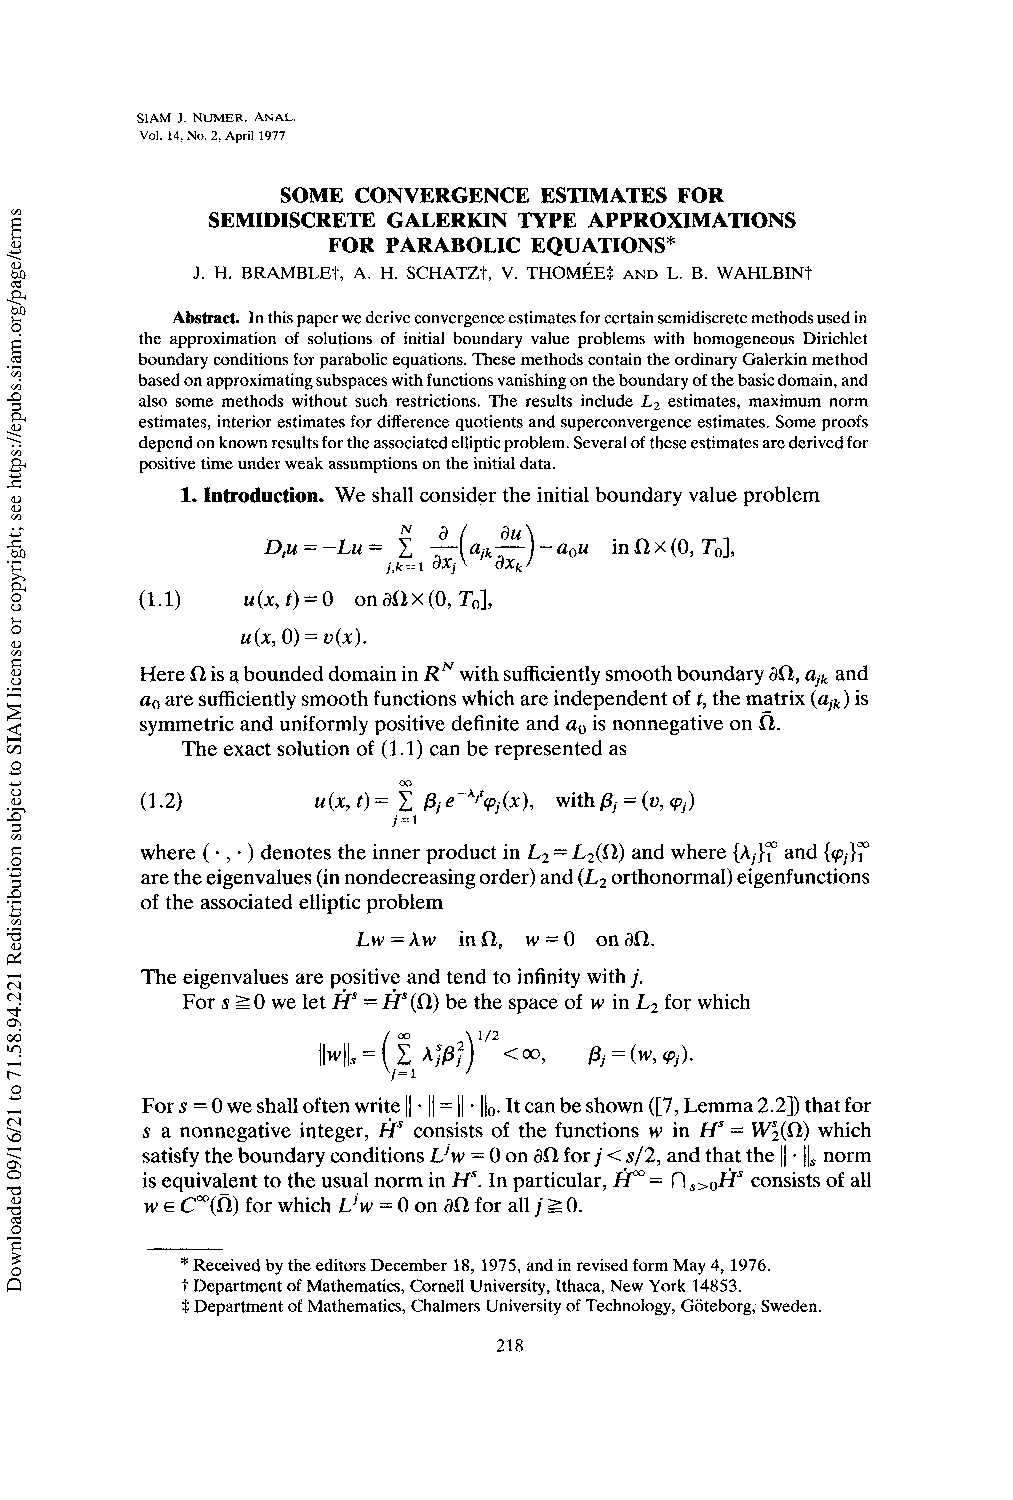
\includepdf[pages = -]{Papers/FEM/bramble1977some.pdf}


\section{Semidiscrete and single step fully discrete approximations for second order hyperbolic equations (1979)}
\cite{baker1979semidiscrete}
\includepdf[pages = -]{Papers/FEM/baker1979semidiscrete.pdf}


\section{Some estimates for a weighted $L^2$ projection (1991)}
Some estimates for a weighted $L^2$ projection\cite{bramble1991some}
\includepdf[pages = -]{Papers/FEM/bramble1991some.pdf}

\section{On variational formulations for the Stokes equations with nonstandard boundary conditions (1994)}
On variational formulations for the Stokes equations with nonstandard boundary conditions\cite{bramble1994variational}
\includepdf[pages = -]{Papers/FEM/bramble1994variational.pdf}


\section{A finite element method for interface problems in domains with smooth boundaries and interfaces (1996)}
A finite element method for interface problems in domains with smooth boundaries and interfaces\cite{bramble1996finite}
\includepdf[pages = -]{Papers/FEM/bramble1996finite.pdf}



\section{New interpolation results and applications to finite element methods for elliptic boundary value problems (2001)}
New interpolation results and applications to finite element methods for elliptic boundary value problems\cite{bacuta2001new}
\includepdf[pages = -]{Papers/FEM/bacuta2001new.pdf}


\section{On the stability of the L2 projection in $H^1(\Omega)$ (2002)}
On the stability of the L2 projection in $H^1(\Omega)$\cite{bramble2002stability}
\includepdf[pages = -]{Papers/FEM/bramble2002stability.pdf}

\section{A proof of the inf--sup condition for the Stokes equations on Lipschitz domains (2003)}
A proof of the inf--sup condition for the Stokes equations on Lipschitz domains\cite{bramble2003proof}
\includepdf[pages = -]{Papers/FEM/bramble2003proof.pdf}

\section{Using finite element tools in proving shift theorems for elliptic boundary value problems (2003)}
Using finite element tools in proving shift theorems for elliptic boundary value problems\cite{bacuta2003using}
\includepdf[pages = -]{Papers/FEM/bacuta2003using.pdf}


\section{Super-convergence}

\subsection{Higher order local accuracy by averaging in the finite element method (1977)}
Higher order local accuracy by averaging in the finite element method\cite{bramble1977higher}
\includepdf[pages = -]{Papers/FEM/bramble1977higher.pdf}

\subsection{A local post-processing technique for improving the accuracy in mixed finite-element approximations (1989)}
A local post-processing technique for improving the accuracy in mixed finite-element approximations\cite{bramble1989local}
\includepdf[pages = -]{Papers/FEM/bramble1989local.pdf}


%\subsection{A local post-processing technique for improving the accuracy in mixed finite-element approximations}
%A local post-processing technique for improving the accuracy in mixed finite-element approximations \cite{bramble1989local}.
%\includepdf[pages = -]{Papers/FEM/bramble1989local.pdf}

%\subsection{Higher order local accuracy by averaging in the finite element method}
%Higher order local accuracy by averaging in the finite element method \cite{bramble1977higher}.
%\includepdf[pages = -]{Papers/FEM/bramble1977higher.pdf}



%\input{ArticleCollection/Tex/SuperC.tex}
%\chapter{Domain Decomposition Methods}
\chapter{Multigrid Methods}


\section{New convergence estimates for multigrid algorithms (1987)}
New convergence estimates for multigrid algorithms\cite{bramble1987new}
\includepdf[pages = -]{Papers/MG/bramble1987new.pdf}

\section{The analysis of multigrid algorithms for nonsymmetric and indefinite elliptic problems (1988)}
The analysis of multigrid algorithms for nonsymmetric and indefinite elliptic problems\cite{bramble1988analysis}
\includepdf[pages = -]{Papers/MG/bramble1988analysis.pdf}

\section{Parallel multilevel preconditioners (1990)}
New convergence estimates for multigrid algorithms\cite{bramble1990parallel}
\includepdf[pages = -]{Papers/MG/bramble1990parallel.pdf}

\section{The analysis of multigrid algorithms with nonnested spaces or noninherited quadratic forms (1991)}
The analysis of multigrid algorithms with nonnested spaces or noninherited quadratic forms\cite{bramble1991analysis}
\includepdf[pages = -]{Papers/MG/bramble1991analysis.pdf}

\section{Convergence estimates for multigrid algorithms without regularity assumptions (1991)}
Convergence estimates for multigrid algorithms without regularity assumptions\cite{bramble1991convergence-a}
\includepdf[pages = -]{Papers/MG/bramble1991convergence.pdf}

\section{The analysis of smoothers for multigrid algorithms (1992)}
The analysis of smoothers for multigrid algorithms\cite{bramble1992analysis}
\includepdf[pages = -]{Papers/MG/bramble1992analysis.pdf}

\section{New estimates for multilevel algorithms including the V-cycle (1993)}
New estimates for multilevel algorithms including the V-cycle\cite{bramble1993new}
\includepdf[pages = -]{Papers/MG/bramble1993new.pdf}

\section{The analysis of multigrid algorithms for pseudodifferential operators of order minus one (1994)}
The analysis of multigrid algorithms for pseudodifferential operators of order minus one\cite{bramble1994analysis}
\includepdf[pages = -]{Papers/MG/bramble1994analysis.pdf}

\section{Uniform convergence of multigrid V-cycle iterations for indefinite and nonsymmetric problems (1994) }
Uniform convergence of multigrid V-cycle iterations for indefinite and nonsymmetric problems\cite{bramble1994uniforma}
\includepdf[pages = -]{Papers/MG/bramble1994uniform.pdf}


\section{Uniform Convergence Estimates for Multigrid V-cycle Algorithms with Less than Full Elliptic Regularity (1994)}
Uniform Convergence Estimates for Multigrid V-cycle Algorithms with Less than Full Elliptic Regularity\cite{bramble1994uniformb}
\includepdf[pages = -]{Papers/MG/bramble1994uniform-bramble.pdf}


\section{Interpolation between Sobolev spaces in Lipschitz domains with an application to multigrid theory (1995)}
Interpolation between Sobolev spaces in Lipschitz domains with an application to multigrid theory\cite{bramble1995interpolation}
\includepdf[pages = -]{Papers/MG/bramble1995interpolation.pdf}


\section{Multigrid methods for the biharmonic problem discretized by conforming $C^1$ finite elements on nonnested meshes (1995)}
Multigrid methods for the biharmonic problem discretized by conforming $C^1$ finite elements on nonnested meshes\cite{bramble1995multigrid}
\includepdf[pages = -]{Papers/MG/bramble1995multigrid.pdf}



\section{The analysis of multigrid algorithms for cell centered finite difference methods (1996)}
The analysis of multigrid algorithms for cell centered finite difference methods\cite{bramble1996analysis}
\includepdf[pages = -]{Papers/MG/bramble1996analysis.pdf}


%\section{The analysis of multigrid methods (2000)}
%The analysis of multigrid methods\cite{bramble2000analysis}
%\includepdf[pages = -]{Papers/MG/bramble2000analysis.pdf}

\section{Uniform convergence of the multigrid V-cycle for an anisotropic problem (2001)}
Uniform convergence of the multigrid V-cycle for an anisotropic problem\cite{bramble2001uniform}
\includepdf[pages = -]{Papers/MG/bramble2001uniform.pdf}












%\chapter{Domain Decomposition Methods}
%\section{Non-overlapping domain decomposition methods}
%\begin{enumerate}
%\item An iterative method for elliptic problems on regions partitioned into substructures
%\item The construction of preconditioners for elliptic problems by substructuring. I
%\item The construction of preconditioners for elliptic problems by substructuring. II
%\item The construction of preconditioners for elliptic problems by substructuring. III 
%\item The construction of preconditioners for elliptic problems by substructuring. IV 
%\end{enumerate}
%
%\section{Overlapping domain decomposition methods}
%\begin{enumerate}
%\item Convergence estimates for product iterative methods with applications to domain decomposition
%\end{enumerate}

\chapter{Domain Decomposition Methods}
\section{The construction of preconditioners for elliptic problems by substructuring. I (1986)}
The construction of preconditioners for elliptic problems by substructuring. I \cite{bramble1986construction}
\includepdf[pages = -]{Papers/DDM/bramble1986construction.pdf}

\section{The construction of preconditioners for elliptic problems by substructuring. II (1987)}
The construction of preconditioners for elliptic problems by substructuring. II\cite{bramble1987construction}
\includepdf[pages = -]{Papers/DDM/bramble1987construction.pdf}

\section{The construction of preconditioners for elliptic problems by substructuring. III (1988)}
The construction of preconditioners for elliptic problems by substructuring. III \cite{bramble1988construction}
\includepdf[pages = -]{Papers/DDM/bramble1988construction.pdf}

\section{The construction of preconditioners for elliptic problems by substructuring. IV (1989)}
The construction of preconditioners for elliptic problems by substructuring. IV \cite{bramble1989construction}
\includepdf[pages = -]{Papers/DDM/bramble1989construction.pdf}

\section{An iterative method for elliptic problems on regions partitioned into substructures (1986)}
An iterative method for elliptic problems on regions partitioned into substructures \cite{bramble1986construction}
\includepdf[pages = -]{Papers/DDM/bramble1986iterative.pdf}

\section{A domain decomposition technique for Stokes problems (1990)}
A domain decomposition technique for Stokes problems \cite{bramble1990domain}
\includepdf[pages = -]{Papers/DDM/bramble1990domain.pdf}

\section{Convergence estimates for product iterative methods with applications to domain decomposition (1991)}
Convergence estimates for product iterative methods with applications to domain decomposition \cite{bramble1991convergence-b}
\includepdf[pages = -]{Papers/DDM/bramble1991convergence-bramble.pdf}

\section{Domain decomposition methods for problems with uniform local refinement in two dimensions (1991)}
Domain decomposition methods for problems with uniform local refinement in two dimensions \cite{bramble1991domain}
\includepdf[pages = -]{Papers/DDM/bramble1991domain.pdf}

\section{Domain decomposition methods for problems with partial refinement (1992)}
Domain decomposition methods for problems with partial refinement \cite{bramble1992domain}
\includepdf[pages = -]{Papers/DDM/bramble1992domain.pdf}

\section{Analysis of non-overlapping domain decomposition algorithms with inexact solves (1998)}
Analysis of non-overlapping domain decomposition algorithms with inexact solves \cite{bramble1998analysis}
\includepdf[pages = -]{Papers/DDM/bramble1998analysis.pdf}


\chapter{Least-squares Methods}

\section{Least squares methods for 2$m$th order elliptic boundary-value problems (1971)}
Least squares methods for 2$m$th order elliptic boundary-value problems \cite{bramble1971least}
\includepdf[pages = -]{Papers/LS/bramble1971least.pdf}


\section{On the numerical solution of elliptic boundary value problems by least squares approximation of the data (1971)}
On the numerical solution of elliptic boundary value problems by least squares approximation of the data \cite{bramble1971numerical}
\includepdf[pages = -]{Papers/LS/bramble1971numerical.pdf}


\section{Semidiscrete least-squares methods for a parabolic boundary value problem (1972)}
Semidiscrete least-squares methods for a parabolic boundary value problem \cite{bramble1972semidiscrete}
\includepdf[pages = -]{Papers/LS/bramble1972semidiscrete.pdf}


\section{A generalized Ritz-least-squares method for Dirichlet problems (1973)}
A generalized Ritz-least-squares method for Dirichlet problems \cite{bramble1973generalized}
\includepdf[pages = -]{Papers/LS/bramble1973generalized.pdf}


\section{Least-squares methods for Stokes equations based on a discrete minus one inner product (1996)}
Least-squares methods for Stokes equations based on a discrete minus one inner product \cite{bramble1996least}
\includepdf[pages = -]{Papers/LS/bramble1996least.pdf}


\section{A least-squares approach based on a discrete minus one inner product for first order systems (1997)}
A least-squares approach based on a discrete minus one inner product for first order systems \cite{bramble1997least}
\includepdf[pages = -]{Papers/LS/bramble1997least.pdf}


\section{Least-squares for second-order elliptic problems (1998)}
Least-squares for second-order elliptic problems \cite{bramble1998least}
\includepdf[pages = -]{Papers/LS/bramble1998least.pdf}


\section{A negative-norm least squares method for Reissner-Mindlin plates (1998)}
A negative-norm least squares method for Reissner-Mindlin plates \cite{bramble1998negative}
\includepdf[pages = -]{Papers/LS/bramble1998negative.pdf}


\section{Least-squares methods for linear elasticity based on a discrete minus one inner product (2001)}
Least-squares methods for linear elasticity based on a discrete minus one inner product \cite{bramble2001least}
\includepdf[pages = -]{Papers/LS/bramble2001least.pdf}


\section{The approximation of the Maxwell eigenvalue problem using a least-squares method (2005)}
The approximation of the Maxwell eigenvalue problem using a least-squares method \cite{bramble2005approximation}
\includepdf[pages = -]{Papers/LS/bramble2005approximation.pdf}


\section{A least-squares approximation method for the time-harmonic Maxwell equations (2005)}
A least-squares approximation method for the time-harmonic Maxwell equations \cite{bramble2005least}
\includepdf[pages = -]{Papers/LS/bramble2005least.pdf}



\chapter{PML Methods}

\section{Analysis of a finite PML approximation for the three dimensional time-harmonic Maxwell and acoustic scattering problems (2007)}
Analysis of a finite PML approximation for the three dimensional time-harmonic Maxwell and acoustic scattering problems\cite{bramble2007analysis}
\includepdf[pages = -]{Papers/PML/bramble2007analysis.pdf}


\section{Analysis of a finite element PML approximation for the three dimensional time-harmonic Maxwell problem (2008)}
Analysis of a finite element PML approximation for the three dimensional time-harmonic Maxwell problem \cite{bramble2008analysis}
\includepdf[pages = -]{Papers/PML/bramble2008analysis.pdf}



\section{Analysis of a finite PML approximation to the three dimensional elastic wave scattering problem (2010)}
Analysis of a finite PML approximation to the three dimensional elastic wave scattering problem \cite{bramble2010analysis}
\includepdf[pages = -]{Papers/PML/bramble2010analysis.pdf}


\section{Analysis of a Cartesian PML approximation to acoustic scattering problems in $R^2$ and $R^3$ (2010)}
Analysis of a Cartesian PML approximation to acoustic scattering problems in $R^2$ and $R^3$ \cite{bramble2013analysis}
\includepdf[pages = -]{Papers/PML/bramble2013analysis.pdf}
\chapter{Others}

%\section{Some inequalities for vector functions with applications in elasticity (1962)}
%Some inequalities for vector functions with applications in elasticity\cite{bramble1962some}
%\includepdf[pages = -]{Papers/Others/bramble1962some.pdf}

\bibliographystyle{plain}
\bibliography{ArticleCollection/bramble.bib}
%\bibliography{bramble-DDM.bib, bramble-FDM.bib, bramble-FEM.bib, bramble-PML.bib, bramble-MG.bib, bramble-LS.bib, bramble-others.bib}

\end{document}
